%!TEX root = ../dissertation.tex
% \begin{savequote}[75mm]
% 	\itshape Write programs that do one thing and do it well. \\
% 	\itshape Write programs to work together. \\
% 	\itshape Write programs to handle text streams, \\
% 	\itshape because that is a universal interface.
% 	\qauthor{---Peter H. Salus}
% \end{savequote}

\chapter[Python-based molecular modeling workflows]{Python-based \\
molecular modeling workflows}
\label{chap:05}

\Lettrine{Recruiting} different techniques to compose a multistep protocol is the very essence of multiscale molecular modeling. In addition to the scientific challenge itself, a technical barrier can arise: putting all the software to work together. To solve it, the researcher resorts to accumulated expertise in combining different file formats or, in some fortunate cases, even automating the conversions with scripting languages. Switching from program to program can be confusing and distracting, especially if those programs were not meant to be used together ---a common situation in advanced molecular modeling. In those cases, some might prefer using a single cohesive user experience, normally in the form of a graphical interface (see \autoref{chap:01} for more details). The first part of this chapter will present the Tangram suite, a collection of graphical extensions for UCSF Chimera written in Python and Tk.

Of course, not all tasks benefit equally from a graphical interface. Some can be further improved by providing smart command-line tools. The remaining part of the present chapter will introduce complementary developments designed to improve the workflow and daily routine of computational chemists and molecular modelers alike. Both graphical and command-line developments (including GaudiMM) are presented in table \ref{table:insilichem-suite}.


\begin{table}[hbtp]
	\caption[The full InsiliChem Molecular Modeling software suite]{The full InsiliChem Molecular Modeling software suite.}
	\label{table:insilichem-suite}
	\footnotesize
	\newcolumntype{R}{>{\hsize=.25\hsize\raggedleft\arraybackslash}X}%
	\newcolumntype{L}{>{\hsize=.75\hsize\raggedright\arraybackslash}X}%
	\newcommand{\tableheading}[1]{\multicolumn{2}{c}{\textsc{#1}}}
	\begin{tabularx}{\textwidth}{RL}
		\toprule
		%row no:1
		\tableheading{Graphical interfaces} \\
		\toprule
		%row no:2
		\textsc{Tangram}\cite{tangram} & A collection of more than 15 UCSF Chimera graphical extensions for integrative molecular modeling \\
		\midrule
		%row no:3
		\textsc{ESIgen webUI}\cite{esigen} & Automated generation of Supporting Information HTML5 drag \& drop interface \\
		\toprule
		%row no:4
		\tableheading{Command-line tools} \\
		\toprule
		%row no:5
		\textsc{GaudiMM}\cite{gaudimm} & Modular multi-objective molecular optimization platform  \\
		\midrule
		\textsc{PyChimera}\cite{pychimera} & Use UCSF Chimera modules in any Python 2.7 project  \\
		\midrule
		\textsc{OMMProtocol}\cite{ommprotocol} & GPU-accelerated Molecular Dynamics protocols with OpenMM  \\
		\midrule
		%row no:6
		\textsc{Garleek}\cite{garleek} & Gaussian's ONIOM extended with Tinker MM force fields \\
		\midrule
		%row no:7
		\textsc{ESIgen}\cite{esigen} & Automated generation of Supporting Information documents from the command-line (batch mode) \\
		\midrule
		%row no:8
		\textsc{EasyMECP}\cite{easymecp} & A modern workflow for J. N. Harvey's MECP program\cite{harvey1998} \\
		\bottomrule

	\end{tabularx}
\end{table}


\section{Implementation of a common interactive canvas: Tangram}
% \addcontentsline{toc}{section}{Implementation of a common interactive canvas}

Stemming from the former Midas program, UCSF Chimera is presented as \textit{a highly extensible program for interactive visualization and analysis of molecular structures and related data, including density maps, supramolecular assemblies, sequence alignments, docking results, trajectories, and conformational ensembles}. It consists of an interactive 3D visualizer built on top of C++ core with Python bindings, which is responsible of providing much of that promised \textit{extensibility}. GaudiMM, commented in \autoref{chap:04}, heavily uses UCSF Chimera as a backend library, but being a command-line tool, does not need any graphical interaction.

After developing GaudiView as the results viewer for GaudiMM (see \autoref[section]{section:gaudimm-results} and \autoref[appendix]{appendix:more-tangram}), the potential of having simple but powerful graphical interfaces for common modeling tasks became evident. In this section, we present Tangram, a set of extensions designed to add new pieces to the arsenal of molecular modeling tools already present in UCSF Chimera (see fig. \ref{fig:tangram-funnel}).

\begin{figure}
	\begin{Center}
		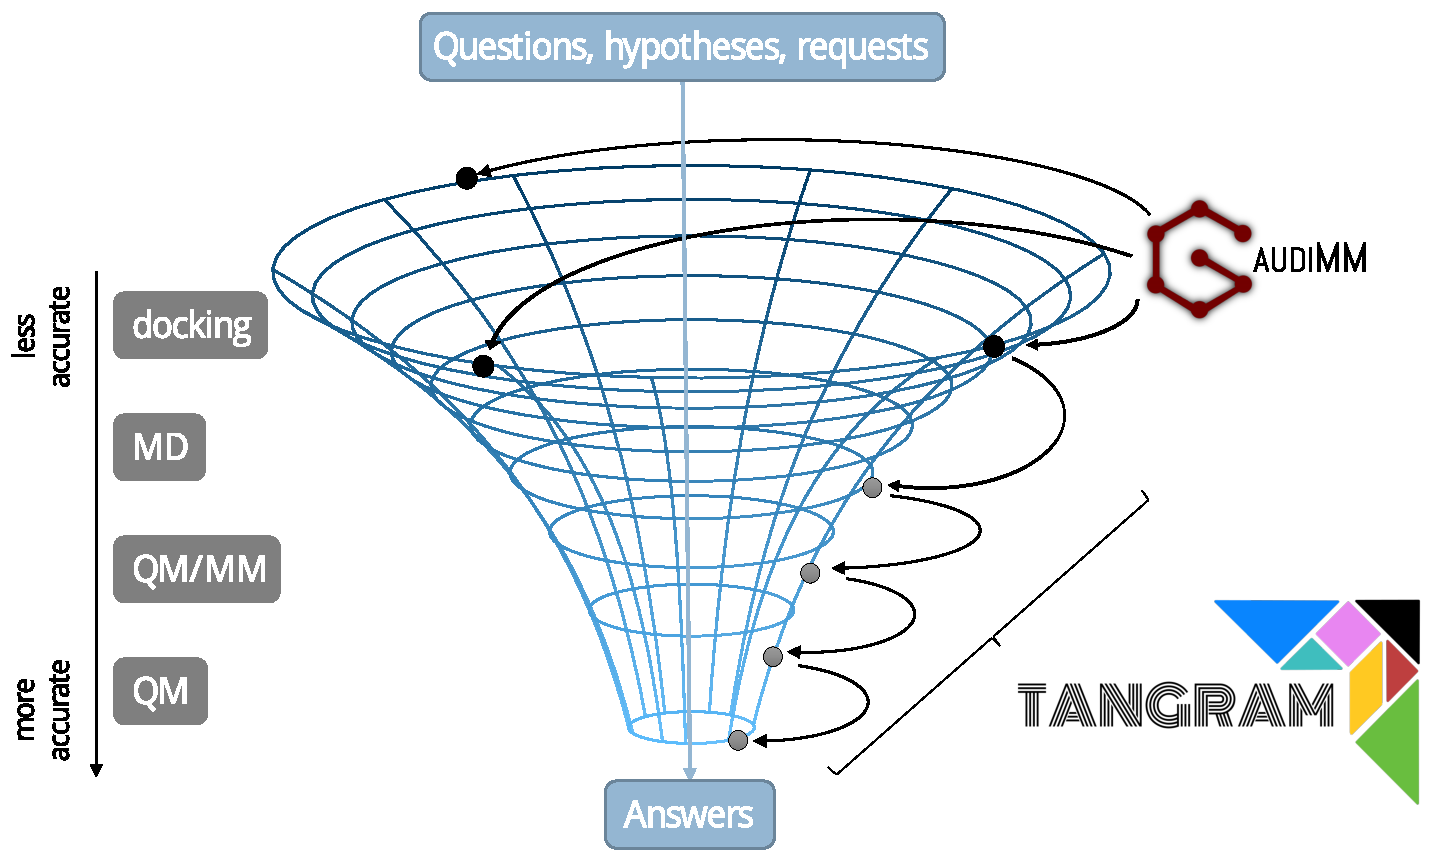
\includegraphics[width=\textwidth]{./figures/05/funnel2.pdf}
	\end{Center}
	\caption[Multiscale funnel]{Molecular modeling methods can be depicted in 3D funnel, where the width represents the sampling capacity and accuracy is depicted with depth. Less accurate methods with high sampling capacity would be depicted at the top, while most accurate methods would be at the bottom of the funnel. In this sense, GaudiMM can help access the entry of the funnel, while the Tangram interfaces will connect further steps down the accuracy scale.}
	\label{fig:tangram-funnel}
\end{figure}


\begin{table}[hbtp]
	\caption[Tangram Suite: Technical datasheet]{Tangram Suite: Technical datasheet.}
	\footnotesize
	\newcolumntype{R}{>{\hsize=.25\hsize\raggedleft\arraybackslash}X}%
	\newcolumntype{L}{>{\hsize=.75\hsize\raggedright\arraybackslash}X}%
	\newcommand{\tableheading}[1]{\multicolumn{2}{c}{\textsc{#1}}}
	\begin{tabularx}{\textwidth}{RL}
		\toprule
		%row no:1
		\tableheading{Tangram Suite}\\
		\toprule
		%row no:2
		\textit{Description} & Graphical interfaces for UCSF Chimera\\
		\midrule
		%row no:3
		\textit{Requirements} & UCSF Chimera, Python, PyChimera\\
		\midrule
		%row no:4
		\textit{License} & MIT\\
		\midrule
		%row no:5
		\textit{Download} & \href{https://github.com/insilichem/tangram}{github.com/insilichem/tangram} \\
		\midrule
		%row no:6
		\textit{Documentation} & \href{http://tangram-suite.readthedocs.io}{tangram-suite.readthedocs.io} \\
		\midrule
		%row no:7
		\textit{Citation} & (Submitted)\\
		\bottomrule

	\end{tabularx}
\end{table}


Tangram is composed of independent UCSF Chimera extensions that can play together through the interactive molecular canvas. This is, each extension can be used separately, but complex workflows can be implemented by using them sequentially. This distantly mimics the principles described in the UNIX philosophy: each extension should only do one thing and do it well.\cite{raymond2003art} As a result, some extensions in this package might look simple, but their true power arises when used together, like the pieces of a tangram puzzle. Hence the name.

The different \textit{tans} or components of Tangram can be of very different nature. Some provide interactive methods for setting up heavy calculations in external programs, like quantum mechanics in Gaussian or molecular dynamics in OpenMM. Others rely on the 3D viewer to depict properties of molecular structures as calculated previously in other software, turning UCSF Chimera in an even more versatile analysis tool. Some will wrap well-known executables meant for standalone usage and present the results in the UCSF Chimera canvas interactively, reducing the entry-barrier substantially. The following subsections will describe the Tangram components developed for multiscale modeling, listing the rationale and features implemented. Examples of integrative protocols using some of them will be provided in \autoref{chap:06}. Additional extensions devoted to integrative analysis are collected in \autoref[appendix]{appendix:more-tangram}. The full list can be consulted in table \ref{table:tangram-suite}.


\begin{table}[hbtp]
	\caption[Full list of Tangram extensions]{Full list of Tangram extensions.}
	\label{table:tangram-suite}
	\footnotesize
	\newcolumntype{R}{>{\hsize=.25\hsize\raggedleft\arraybackslash}X}%
	\newcolumntype{L}{>{\hsize=.75\hsize\raggedright\arraybackslash}X}%
	\newcommand{\tableheading}[1]{\multicolumn{2}{c}{\textsc{#1}}}
	\begin{tabularx}{\textwidth}{RL}
		\toprule
		%row no:1
		\tableheading{Calculation setup for multiscale modeling} \\
		\midrule
		\textsc{QMSetup} & QM and QM/MM calculations setup, with Gaussian\cite{gaussian} and Garleek\cite{garleek} \\[0.6ex]
		\textsc{MMSetup} & Setup MD calculations with OpenMM\cite{openmm} and OMMProtocol\cite{ommprotocol} \\[0.6ex]
		\textsc{DummyMetal} & Parameterize metal ions for MM with the CaDAs\cite{duarte2014} approach by placing dummy atoms in the coordination vertices\\[0.6ex]
		\textsc{NormalModes} & Perform interactive Normal Modes Analysis with ProDy\cite{prody} \\[0.6ex]
		\textsc{ReVina} & Resubmit failed AutoDock Vina\cite{trott2010autodock} jobs without reconfiguring the GUI \\

		\midrule
		\tableheading{Interaction analysis} \\
		\midrule

		\textsc{GaudiView} & Lightweight visualization of results coming from GaudiMM\cite{gaudimm} and GOLD\cite{gold} \\[0.6ex]
		\textsc{NCIPlotGUI} & Setup calculations for NCIPlot\cite{nciplot} and visualize them on-screen \\[0.6ex]
		\textsc{PLIPGUI} & Depict protein-ligand interactions, as calculated with PLIP\cite{salentin2015plip} \\

		%row no:5
		\midrule
		\tableheading{Structural analysis} \\
		\midrule
		\textsc{3D-SNFG} & Intuitive visualization of saccharydic residues with the Symbol Nomenclature For Glycans\cite{snfg,3dsnfg} \\[0.6ex]
		\textsc{OrbiTraj} & Display temporal volumetric data along a molecular trajectory \\[0.6ex]
		\textsc{PoPMuSiCGUI} & Depict potential site mutations in proteins as predicted by PoPMuSiC\cite{dehouck2011popmusic} \\[0.6ex]
		\textsc{PropKaGUI} & Analyze the expected pKa values of protein residues with PropKa 3.1\cite{propka} \\[0.6ex]
		\textsc{SubAlign} & Align potentially different molecules based on partial matches of substructures with RDKit\cite{rdkit} \\
		%row no:5
	\bottomrule

	\end{tabularx}
\end{table}



\subsection{Multiscale modeling with Tangram}


% \addcontentsline{toc}{subsection}{Calculation setup}
\subsubsection{QMSetup}
% \addcontentsline{toc}{subsubsection}{QMSetup}
QMSetup helps prepare Gaussian input files from UCSF Chimera for QM and ONIOM calculations (see \autoref[sections]{section:qm} and \autoref[]{section:qmmm}). In GaussView,\cite{gaussview} setting up even the most common tasks would require going through scattered dialogs and tabs. QMSetup has been designed to provide a simpler workflow from a single dialog. Additionally, while UCSF Chimera is not as intuitive as GaussView for building small molecules, with QMSetup it shows several usability advantages, especially when macromolecules are present. Some highlights include:

\begin{itemize}
	\item In UCSF Chimera, selection commands are hierarchical and can be extended from atoms to residues, chains and subunits with a single key stroke. This is really useful for selecting layers in ONIOM jobs or choosing which atoms should be frozen in an optimization, both options present in QMSetup.

	\item Some multiscale protocols involve setting up QM/MM jobs from different frames of a molecular dynamics trajectories. The different frames are just different coordinates sets of the same topology, so instead of creating separate input files one by one, a single one needs to be created. The remaining ones can be created automatically by updating the first one with the adequate coordinates. This is possible with QMSetup \textit{Replica} option.

	\item In organometallics, exotic elements are used frequently. For these species, special basis sets are usually needed. Advanced users know about the Basis Set Exchange (BSE)\cite{schuchardt2007basis} online platform and use it to locate the needed basis sets. QMSetup provides an offline interface to this dataset and handles the insertion in the input file automatically. This saves the hassle of copy-pasting the results and worrying about the adequate number of blank lines.
\end{itemize}



\begin{figure}
	\begin{Center}
		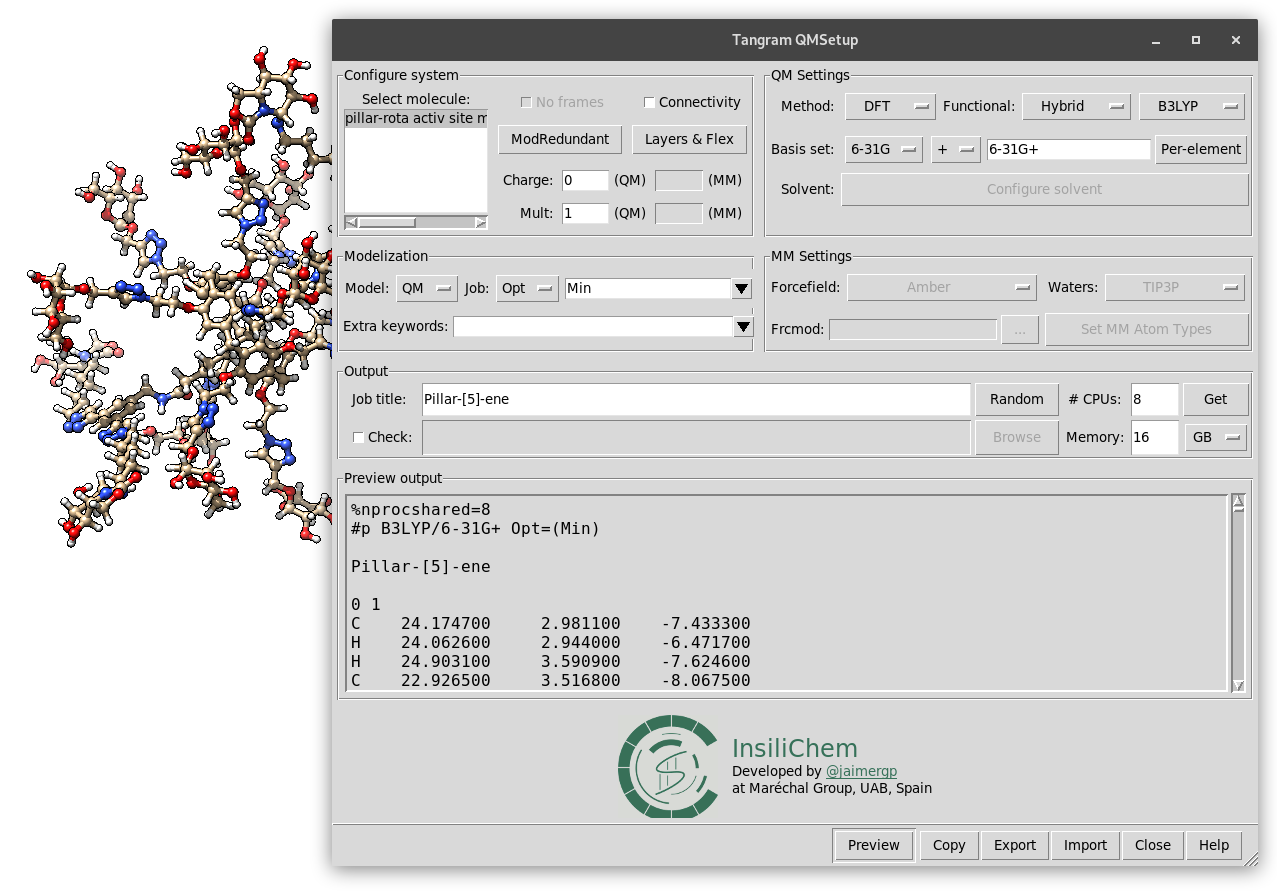
\includegraphics[width=\textwidth]{./figures/05/tangram_qm.png}
	\end{Center}
	\caption[Tangram QMSetup]{Tangram QMSetup interface allows to create QM and ONIOM jobs for Gaussian.}
	\label{fig:tangram-qmsetup}
\end{figure}


\subsubsection{MMSetup}
% \addcontentsline{toc}{subsubsection}{MMSetup}
MMSetup provides a graphical interface for setting up Molecular Dynamics simulations (see \autoref[section]{section:mm-md})  in UCSF Chimera using OpenMM behind the scenes. It recognizes opened molecules and offers different methods to prepare the final structure that will undergo the simulation (see fig. \ref{fig:tangram-mmsetup}). For example, OpenMM's PDBFixer\cite{pdbfixer} can be used to add hydrogens and missing residues. Even missing loops can be modeled with this integration. Once the structure is prepared, the simulation protocol must be configured with its individual stages: minimization, equilibration and production by default. Then, the user can choose between running in situ and observing the evolution in real time (ideal for educational purposes) or creating an input file that can be run separately in cluster computers for speed.

\begin{figure}
	\begin{Center}
		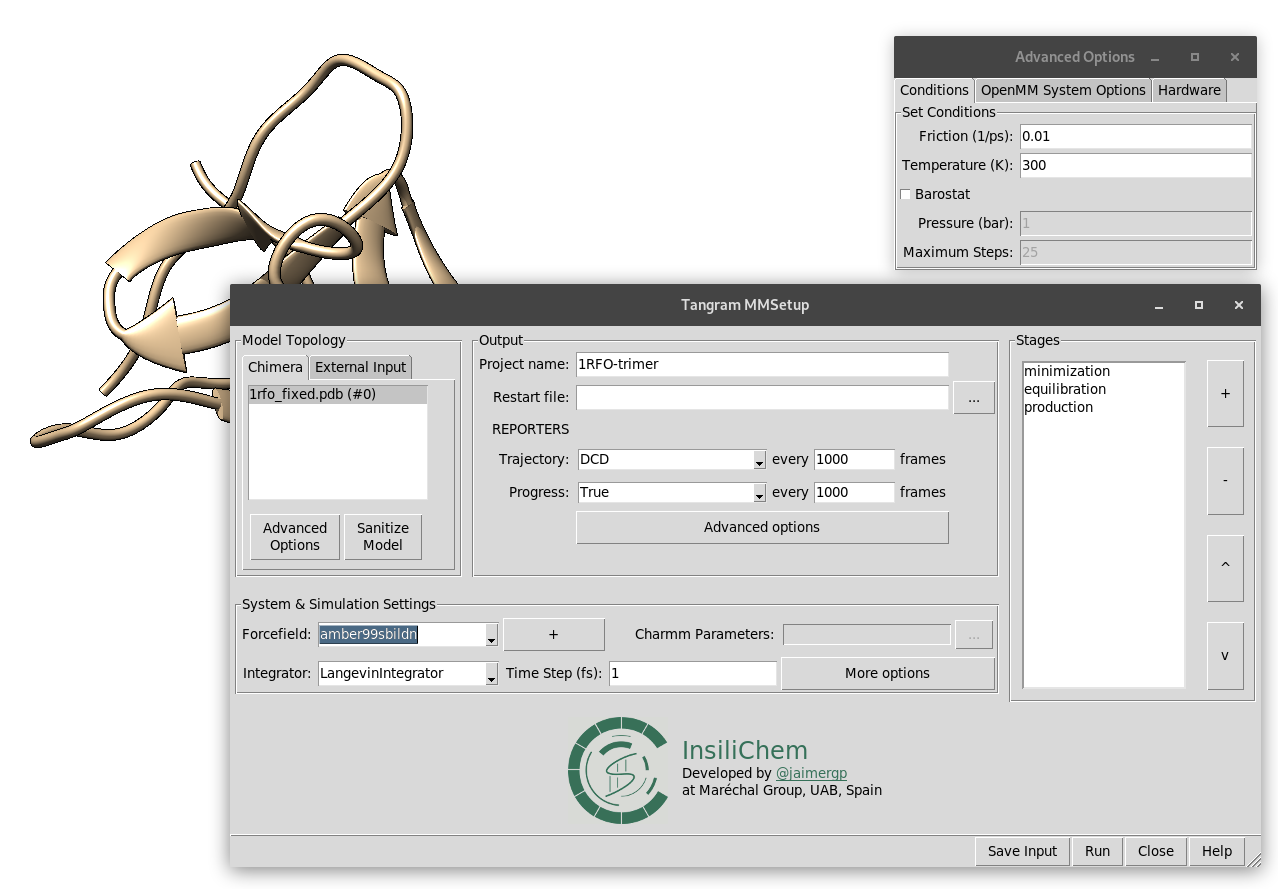
\includegraphics[width=\textwidth]{./figures/05/tangram_mm.png}
	\end{Center}
	\caption[Tangram MMSetup]{Tangram MMSetup can configure OpenMM calculations in UCSF Chimera, which can be run directly on-screen or in a separate job.}
	\label{fig:tangram-mmsetup}
\end{figure}


\subsubsection{DummyMetal}
% \addcontentsline{toc}{subsubsection}{DummyMetal}
In Molecular Mechanics, dealing with residues foreign to default force fields is one of the most difficult tasks. They require custom parameterization that in some cases can involve more complex calculations than the Molecular Dynamics simulation itself. When they are obtained, it is difficult to reuse them in other structures that also feature that residue because the connectivity or oxidation state might have changed. This is particularly painful if the new residue contains a metallic species.

For non-metallic organic compounds, Antechamber\cite{wang2001antechamber} routines are usually enough. However, for metal ions, the process is more intricate. Most methods proposed to generalize this process use high-level calculations in a reduced model, like Seminario's method derived MCPB.py routines,\cite{mcpbpy} but there are alternatives that skip those calculations by implementing virtual positions around the metal ion: the \textit{Cationic Dummy Atoms} (CaDAs) approach.\cite{duarte2014}

In the CaDAs approach, the metal ion is wrapped with positively-charged dummy atoms placed at the vertices of its expected coordination geometry. While the main idea is simple, building these systems accurately by hand is often disregarded for its difficulty. The DummyMetal extension can take a molecular structure, adapt the metal center with the CaDAs method (see fig. \ref{fig:tangram-dummy}) and generate Amber-compatible \texttt{PRMTOP}, \texttt{INPCRD} and \texttt{FRCMOD} files. Since OpenMM can load Amber files seamlessly, the resulting files can be loaded in MMSetup to launch an MD simulation right away.

\begin{figure}
	\begin{Center}
		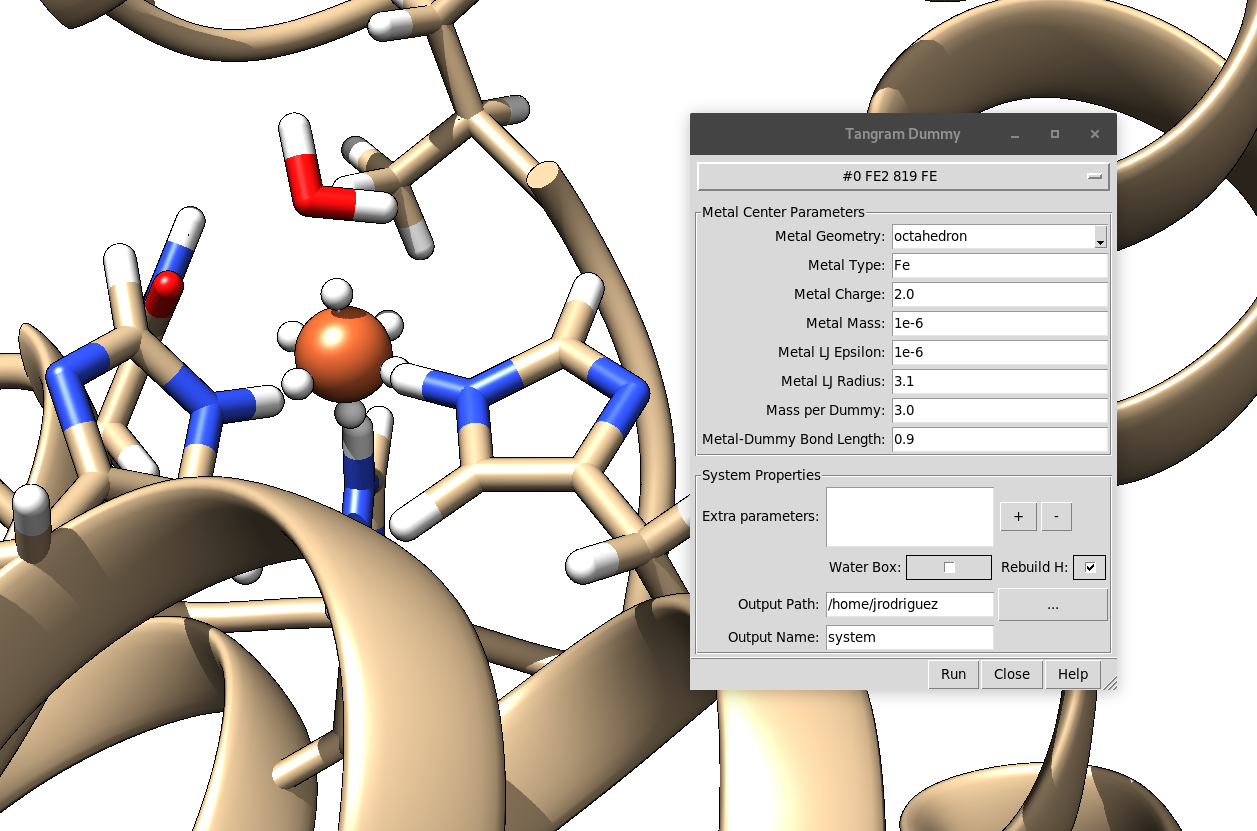
\includegraphics[width=\textwidth]{./figures/05/tangram_dummy.png}
	\end{Center}
	\caption[Tangram DummyMetal]{With Tangram DummyMetal, metal centers can be easily modeled in MM force fields by following the CaDAs approach.}
	\label{fig:tangram-dummy}
\end{figure}

\subsubsection{NormalModes}
% \addcontentsline{toc}{subsubsection}{NormalModes}
Normal Modes Analysis methods are routinely used to study structural dynamics of molecules. Structural variability can be inferred from experimental data or computed MD simulations with principal component analysis (PCA), but it can be also computed with elastic network models (ENM) like the Gaussian or anisotropic network models (GNM and ANM, respectively).

This extension reuses part of the visualization functionality already implemented in UCSF Chimera extensions previously developed by Muñoz Robles,\cite{MunozRobles2014a} but ditches MMTK\cite{mmtk} and calculates ENMs with ProDy,\cite{prody} a more modern Python library specifically designed to compute protein dynamics. The resulting interface will list the calculated frequency vectors and animate the corresponding collective movements.

Since the interface itself is decoupled from the code that calls ProDy routines in the background, the collective vectors can be obtained from Gaussian QM \texttt{freq} jobs as well, if desired.


\section{Optimizing workflows from the command-line}
% \addcontentsline{toc}{section}{Optimizing workflows from the command-line}
While a graphic interface can help with interactive tasks, there are other parts of the workflow of a molecular modeler that cannot benefit directly from a GUI. This type of software can be regarded as \textit{backend} code that provides new, unsupervised calculation methods or, in other cases, an improved workflow that allows to perform the same calculation in an easier way.

Conceiving a project for command-line usage does not mean that a different interface can be built on top of that backend. In fact, MMSetup is just an interface around OMMProtocol, which in turn it's a user-friendly application around OpenMM. In QMSetup, the QM/MM support for additional force fields is provided by Garleek, which handles the Gaussian-Tinker programmatic interfacing. These two tools ---OMMProtocol and Garleek--- do not rely on UCSF Chimera and can be used as standalone command-line applications. However, since they are built with a decoupled architecture where the Python API is separate from the command-line interface (see fig. \ref{fig:uncoupled-layers}), they can support the aforementioned graphical interfaces.

\begin{figure}
	\begin{Center}
		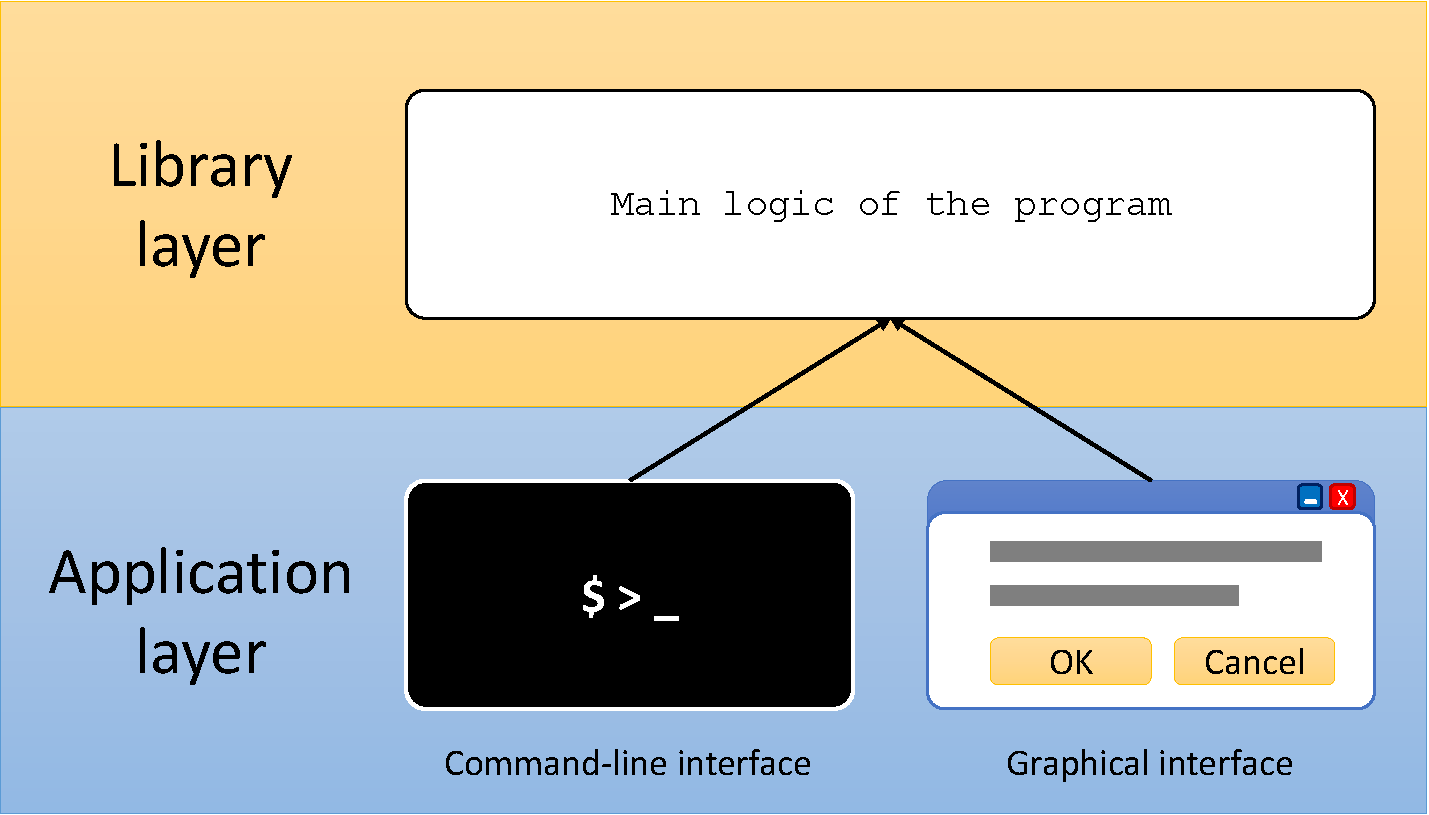
\includegraphics[width=\textwidth]{./figures/05/library-vs-app-layers-crop.pdf}
	\end{Center}
	\caption[Uncoupled software architecture]{By structuring code in separate responsibility layers, new interfaces can be added easily without modifying the core logic.}
	\label{fig:uncoupled-layers}
\end{figure}

In this section, the motivation, features and implementation of five different packages will be discussed: (1) PyChimera, (2) OMMProtocol, (3) Garleek, (4) ESIgen, and (5) EasyMECP. Unlike GaudiMM, discussed in the previous chapter, they do not provide novel molecular modeling methods, but they do make them easier to use by automating repetitive tasks or abstracting away the technical details. This, ultimately, ends up saving the user some precious time.

\subsection{PyChimera}
% \addcontentsline{toc}{subsection}{PyChimera behind the scenes}
\label{section:pychimera}

Most of the extensions listed in the previous section relies on libraries developed by 3\textsuperscript{rd} parties that are not present in the UCSF Chimera Python distribution. Installing new packages inside UCSF Chimera is possible, but not very straight-forward. Additionally, some packages required by Tangram need long compilation times that would constitute a high entry barrier. To ease the process, the full Tangram suite can be installed with a single executable that is available in the central code repository.\footnote{\url{https://github.com/insilichem/tangram/releases}}

This is possible thanks to the \texttt{conda} package manager,\cite{conda} which allows to redistribute compiled libraries and applications easily. However, since both \texttt{conda} and UCSF Chimera provide their own Python 2.7 distribution, they do not play well together. To solve this problem, the preloading code originally present in GaudiMM, which was needed to call the \texttt{gaudi} executable directly from the command-line, was extracted into a separate package and extended to connect UCSF Chimera Python distribution with any other one –--be it the system-provided one, or virtual environments like \texttt{conda}'s or \texttt{pipenv}'s.

This new package was called PyChimera.\cite{pychimera} It does not try to alter the original UCSF Chimera installation; it only allows to load new packages from other locations outside the Chimera installation. For that reason, most Tangram extensions (those with external dependencies) will only work if a patched UCSF Chimera instance is loaded with the special \texttt{tangram} command.

\begin{table}[hbtp]
	\caption[PyChimera: Technical datasheet]{PyChimera: Technical datasheet.}
	\footnotesize
	\newcolumntype{R}{>{\hsize=.25\hsize\raggedleft\arraybackslash}X}%
	\newcolumntype{L}{>{\hsize=.75\hsize\raggedright\arraybackslash}X}%
	\newcommand{\tableheading}[1]{\multicolumn{2}{c}{\textsc{#1}}}
	\begin{tabularx}{\textwidth}{RL}
		\toprule
		%row no:1
		\tableheading{PyChimera}\\
		\toprule
		%row no:2
		\textit{Description} & Import UCSF Chimera modules in external Python projects \\
		\midrule
		%row no:3
		\textit{Requirements} & Python, UCSF Chimera \\
		\midrule
		%row no:4
		\textit{License} & LGPL \\
		\midrule
		%row no:5
		\textit{Download} & \href{https://github.com/insilichem/pychimera}{github.com/insilichem/pychimera} \\
		\midrule
		%row no:6
		\textit{Documentation} & \href{http://pychimera.readthedocs.io}{pychimera.readthedocs.io} \\
		\midrule
		%row no:7
		\textit{Citation} & Bioinf. 2018, 34 (10), pp 1784–1785. DOI: 10.1093/bioinformatics/bty021\cite{pychimera} \\
		\bottomrule

	\end{tabularx}
\end{table}

PyChimera also includes some features particularly useful for developers, like exploring the UCSF Chimera codebase from augmented Python interpreters (IPython,\cite{ipython} Jupyter Notebooks\cite{kluyver2016jupyter}) or providing autocompletions and help messages in advanced text editors (Sublime Text, Visual Studio Code). PyChimera was accepted for publication in \textit{Bioinformatics}\cite{pychimera} and is the most popular package uploaded in the InsiliChem repositories (see fig. \ref{fig:ghstats}).


\begin{figure}[hbtp]
	\begin{Center}
		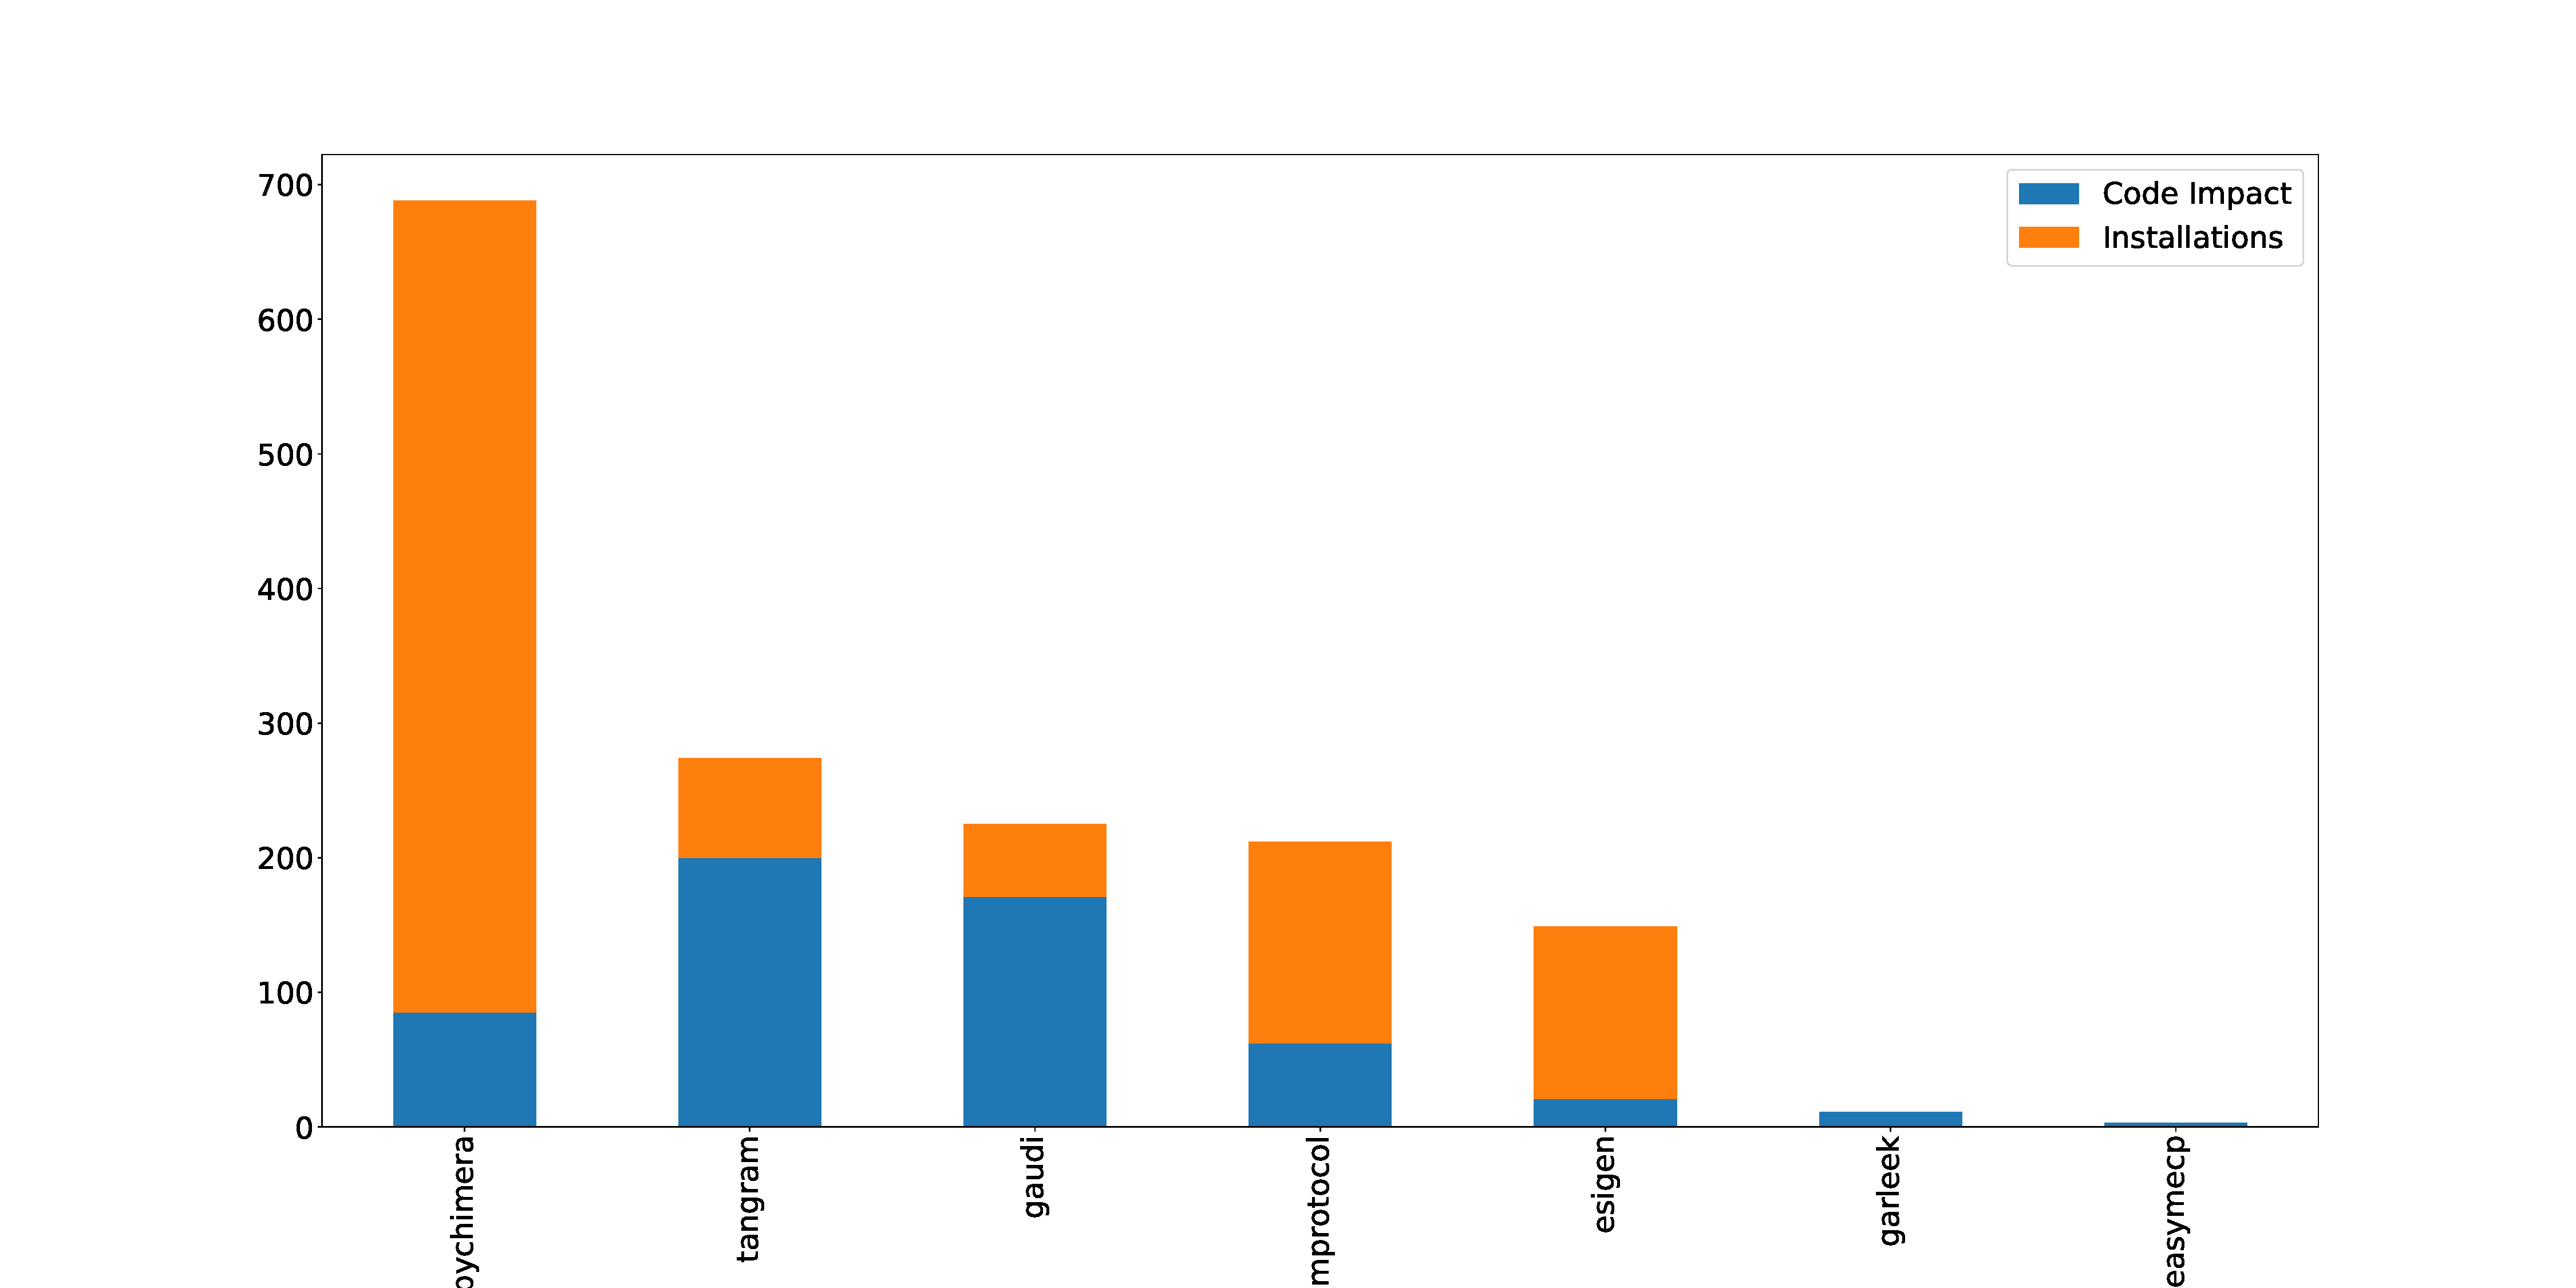
\includegraphics[width=\textwidth]{./figures/05/ghstats.pdf}
	\end{Center}
	\cprotect\caption[Popularity of InsiliChem packages]{Popularity of InsiliChem packages developed during this Ph.D. Thesis, measured as the sum of \textit{Code Impact} (registered visits and interactions in the source code repository), and \textit{Installations} (downloads of compiled packages and requests from command-line installers, such as \texttt{conda} or \texttt{pip}). For ESIgen, number of unique web app users is also listed in Installations. PyChimera is a clear highlight above the rest.}
	\label{fig:ghstats}
\end{figure}


\subsection{GPU-accelerated Molecular Dynamics, the easy way: OMMProtocol}
% \addcontentsline{toc}{subsection}{GPU-accelerated Molecular Dynamics, the easy way: OMMProtocol}
\label{section:ommprotocol}

Molecular Mechanics (MM) and Molecular Dynamics (MD) (see \autoref[section]{section:mm-md}) are widely used in structural biology since they allow observing evolution of large biomolecules along time with affordable timescales and computational resources. This is particularly true after the popularization of General-Purpose Graphic Processing Units (GPGPUs) and their usage for calculations beyond graphics renderization. While long-established MM suites like Amber,\cite{amber} Gromacs\cite{gromacs} or CHARMM\cite{brooks1983} have been progressively implementing GPU acceleration in their code for some years now, a relatively recent project caught the community attention with its performance, flexibility, open-design and availability: the free OpenMM library.\cite{openmm}

OpenMM presents a layered API designed for easy reutilization of its code in other projects. In fact, to use OpenMM, one is expected to write Python scripts to configure the simulation. These scripts are not harder to write that input files for other suites; they just happen to use that scripting language. That said, it could be easier. Users should not need to care about missing parenthesis, import statements or ending quotes. OMMProtocol was conceived to overcome this barrier by providing an easy to read and easy to write input file that abstracts away all the key underlying configuration steps with the concept of \textit{protocol}: each input file contains all the stages involved in the simulation (like minimization, equilibration or production), avoiding the hassle of chained restarts.

\begin{table}[hbtp]
	\caption[OMMProtocol: Technical datasheet]{OMMProtocol: Technical datasheet.}
	\footnotesize
	\newcolumntype{R}{>{\hsize=.25\hsize\raggedleft\arraybackslash}X}%
	\newcolumntype{L}{>{\hsize=.75\hsize\raggedright\arraybackslash}X}%
	\newcommand{\tableheading}[1]{\multicolumn{2}{c}{\textsc{#1}}}
	\begin{tabularx}{\textwidth}{RL}
		\toprule
		%row no:1
		\tableheading{OMMProtocol}\\
		\toprule
		%row no:2
		\textit{Description} & GPU-accelerated Molecular Dynamics simulations \\
		\midrule
		%row no:3
		\textit{Requirements} & Python, OpenMM, ParmEd, MDTraj, openmoltools, pandas, matplotlib, jinja2 \\
		\midrule
		%row no:4
		\textit{License} & LGPL \\
		\midrule
		%row no:5
		\textit{Download} & \href{https://github.com/insilichem/ommprotocol}{github.com/insilichem/ommprotocol} \\
		\midrule
		%row no:6
		\textit{Documentation} & \href{http://ommprotocol.readthedocs.io}{ommprotocol.readthedocs.io} \\
		\midrule
		%row no:7
		\textit{Citation} & (Submitted) \\
		\bottomrule

	\end{tabularx}
\end{table}

With OMMProtocol, setting up GPU-accelerated MD simulations can be as easy as loading a PDB structure, choosing one of the force fields provided and specifying the number of steps. Since default values have been choosing sensibly for compatibility with most popular cases, there is no need for added complication. That said, users are encouraged to review these parameters and adapt them to their specific needs by following the accompanying documentation and input file examples (see fig. \ref{fig:ommprotocol}). More details can be found in the submitted manuscript.\cite{ommprotocol}

OpenMM default input format compatibility is extended with even more file types by integrating other libraries together, like MDTraj,\cite{mdtraj} ParmEd\cite{parmed} or openmoltools.\cite{openmoltools} This means that existing structure preparation workflows do not need to be disrupted: OMMProtocol will load Amber's PRMTOP, Charmm's PSF and Gromacs’ TOP files seamlessly.


\begin{figure}[H] % FIXME!
	\begin{Center}
		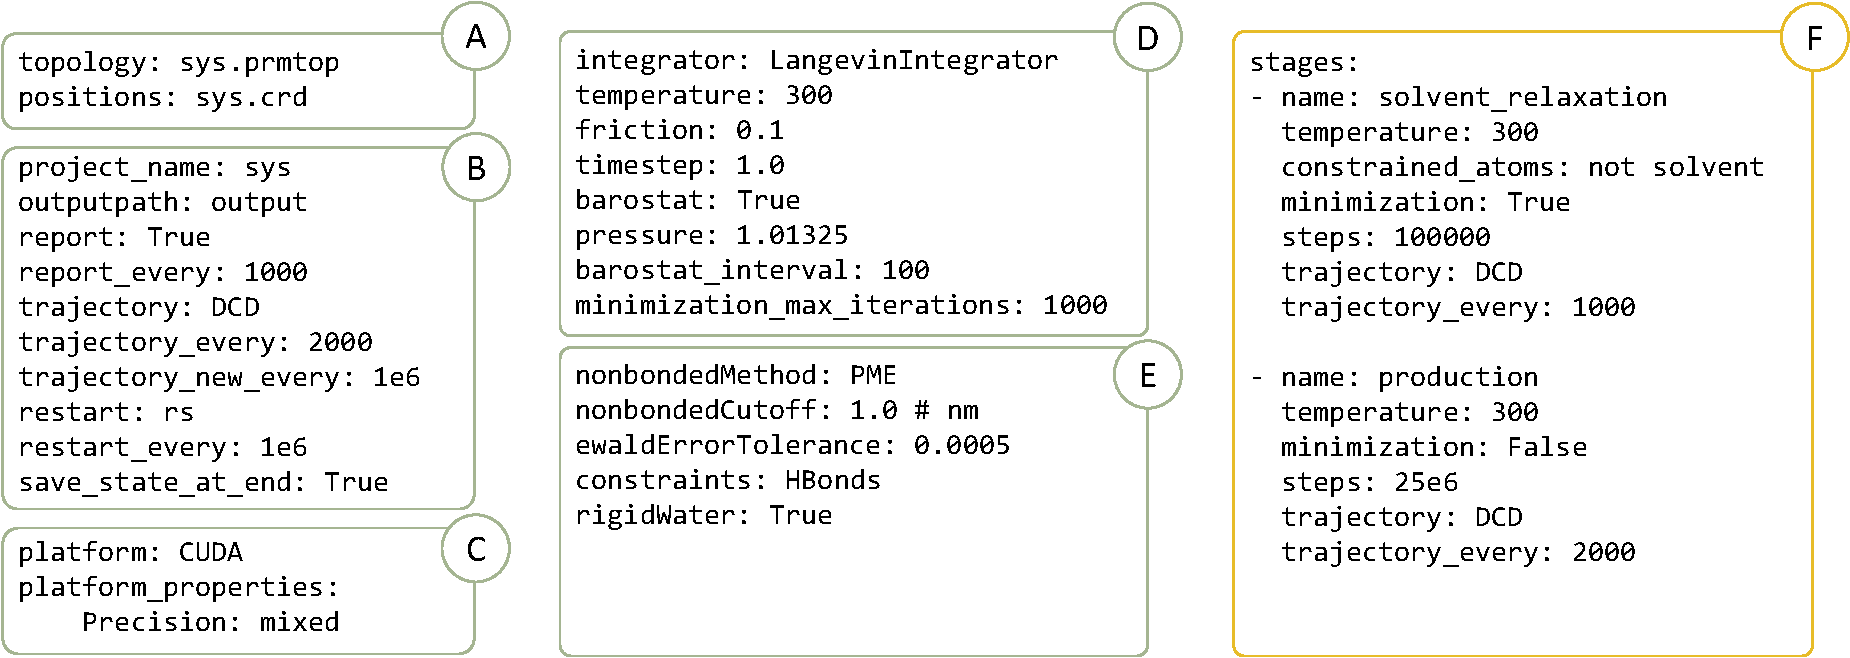
\includegraphics[width=\textwidth]{./figures/05/ommprotocol-crop.pdf}
		\caption[OMMProtocol input file structure]{OMMProtocol files are formatted in YAML. Configuration keys can be specified in any order, but they have been grouped in this figure for convenience. Section A contains the structural data of the system to be simulated: the topology key is always required. Section B groups options related to file output. Section C controls the hardware to be used. Section D and E specify the conditions of the simulation. Finally, section E lists all the stages to be simulated in this protocol. Each entry, marked with a starting dash, can override any of the global options specified in sections B-E. Usually, only constraints, minimization, temperature and simulated steps will be modified here, since every other parameter is normally constant during the full protocol.}
		\label{fig:ommprotocol}
	\end{Center}
\end{figure}


Finally, OMMProtocol is complemented by a second utility called \texttt{ommanalyze}, that drafts support for trajectory analysis protocols following the same spirit as OMMProtocol. This part of the project is only a stub so far, but it already provides automated, constant-memory RMSD analysis, and energy, temperature, and volume plots (see fig. \ref{fig:ommanalyze}).



\begin{figure}[H] % FIXME!
	\begin{Center}
		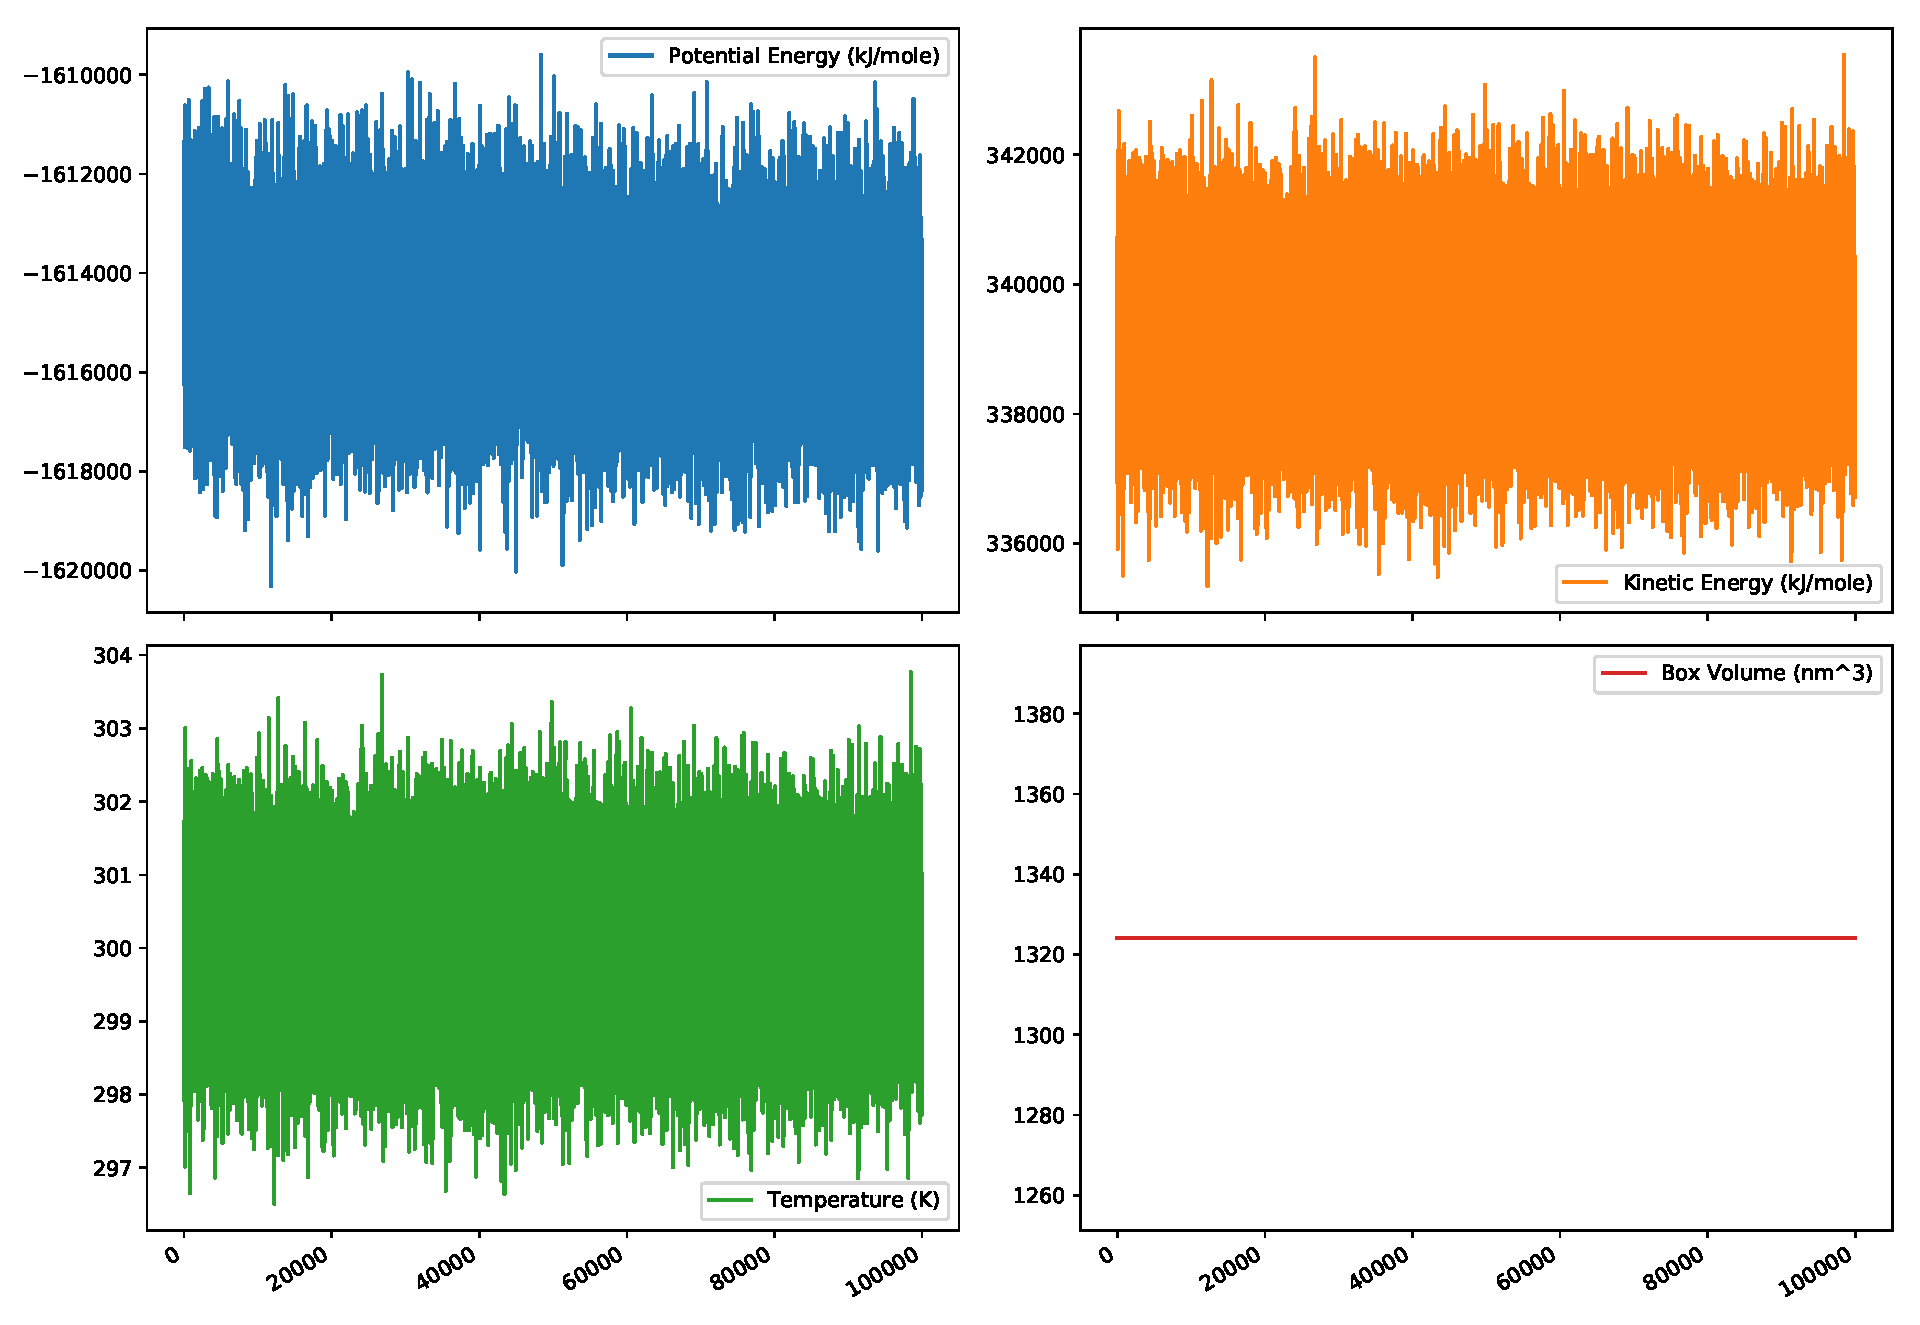
\includegraphics[width=\textwidth]{./figures/05/ommanalyze.pdf}
	\end{Center}
	\caption[Example results with OMMAnalyze]{OMMAnalyze can parse progress reports, written in the background as .log files, to plot the evolution of the potential and kinetic energies, the system temperature and the volume occupied. Since this data is readily available in the .log file, no expensive calculation of the magnitudes is needed. The opened dialog is interactive and can be used to zoom in the data, slice interesting parts and save high-resolution screenshots.}
	\label{fig:ommanalyze}
\end{figure}


\subsection{Extended QM/MM for Gaussian: Garleek}
% \addcontentsline{toc}{subsection}{Extended QM/MM for Gaussian: Garleek}


Gaussian\cite{gaussian} is one of the most popular QM packages and is still actively developed since its first release in the 70s. After almost 50 years, this package has been accumulating more and more features over time, and all of them are requested in the same counter-intuitive input file. While several alternatives exist with a comparable feature set and an easier workflow, even for free,\cite{nwchem} Gaussian is still king on many research groups.

One of the features already included in Gaussian is the ONIOM method,\cite{svensson1996oniom} already described in \autoref{chap:02}. This hybrid method splits a system in layers seeking to combine high-level calculations for specific regions that require very accurate modeling, with low-level theories that will deal with the remaining parts of the system. Most common applications usually use a QM method like DFT for the \textit{high} layer and an MM method for the \textit{low} layer. For this case, Gaussian provides a built-in MM engine suitable for calculations with only three force fields: Amber,\cite{cornell1995second} UFF\cite{Rappe1992} and Dreiding.\cite{Mayo1990} Fortunately, for those users that need other force fields, a communication protocol with 3\textsuperscript{rd} party software is provided through the \texttt{external} keyword.

\begin{table}[hbtp]
	\caption[Garleek: Technical datasheet]{Garleek: Technical datasheet.}
	\footnotesize
	\newcolumntype{R}{>{\hsize=.25\hsize\raggedleft\arraybackslash}X}%
	\newcolumntype{L}{>{\hsize=.75\hsize\raggedright\arraybackslash}X}%
	\newcommand{\tableheading}[1]{\multicolumn{2}{c}{\textsc{#1}}}
	\begin{tabularx}{\textwidth}{RL}
		\toprule
		%row no:1
		\tableheading{Garleek}\\
		\toprule
		%row no:2
		\textit{Description} & Additional MM support for Gaussian ONIOM jobs \\
		\midrule
		%row no:3
		\textit{Requirements} & Gaussian, TINKER, Python, NumPy \\
		\midrule
		%row no:4
		\textit{License} & MIT \\
		\midrule
		%row no:5
		\textit{Download} & \href{https://github.com/insilichem/garleek}{github.com/insilichem/garleek} \\
		\midrule
		%row no:6
		\textit{Documentation} & \href{http://garleek.readthedocs.io}{garleek.readthedocs.io} \\
		\midrule
		%row no:7
		\textit{Citation} & Journal of Computational Chemistry, 2018. (In press) \\
		\bottomrule

	\end{tabularx}
\end{table}

Garleek is a Python package born after a collaboration with Dr. Ignacio Funes and Prof. Feliu Maseras. Garleek is designed to use this protocol to delegate the MM calculations to any other MM suite (see fig. \ref{fig:garleek}). In the present state, it has full compatibility with all TINKER-provided force fields, like Amber99SB,\cite{amber99sb}\footnote{Gaussian does include the Amber forcefield, but an outdated version (94 and 98).} CHARMM,\cite{mackerell1998all} AMOEBA,\cite{amoeba} MMFF\cite{halgren1996merck} or MM3.\cite{allinger1989molecular} Since the underlying architecture implemented in Garleek provides a straight set of guidelines, adding more MM packages is as easy as possible, thus avoiding reinventing the wheel. Garleek has been described in Journal of Computational Chemistry's Special Issue\cite{garleek} dedicated to the memory of Prof. Dr. Keiji Morokuma.



\begin{figure}[H] % FIXME!
	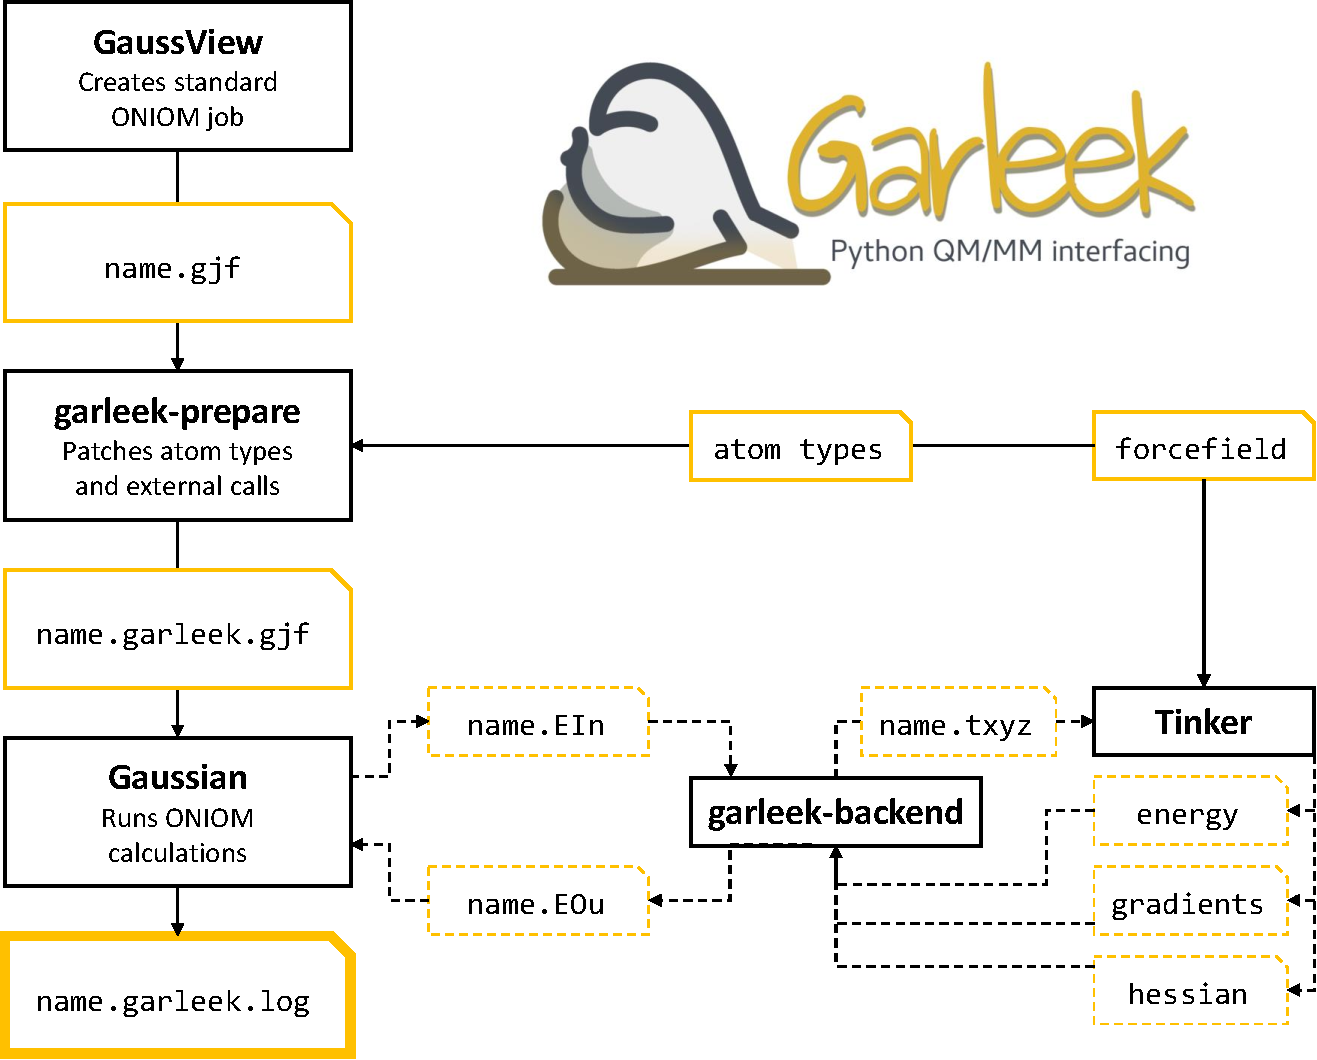
\includegraphics[width=\textwidth]{./figures/05/garleek-crop.pdf}
	\cprotect\caption[ONIOM workflow with Garleek]{ONIOM workflow with Garleek. Black-border boxes describe programs, yellow-border boxes describe files. Dashed borders and lines describe temporary files created and removed on demand. The standard workflow involves creating a standard ONIOM input file (\texttt{name.gjf}) configured which is then patched to be Garleek-compatible with the garleek-prepare command, generating a copy (\texttt{name.garleek.gjf}). Gaussian runs this file and calls garleek-backend when necessary, which handles the communication with Tinker binaries for the MM calculations. The results are written to \texttt{name.garleek.log}.}
	\label{fig:garleek}
\end{figure}


\subsection{Automated Electronic Supporting Information Generator: ESIgen}
% \addcontentsline{toc}{subsection}{Automated Electronic Supporting Information Generator: ESIgen}


Any scientific text must convey well-written ideas that make no room for ambiguous interpretation, but at the same time it should be easy to read. Handling such apparently conflicting ideas with ease is one of the reasons why good scientific communication is considered a hard task. One of the approaches to keeping the reader interested without losing correctness is to maintain a concise and direct style, which usually means taking all the technical details off the main text and supplying them in an accompanying document. Sometimes disregarded, Supporting Information (SI) and its electronic-only variant (ESI) are key to science reproducibility.

Computational chemistry, as all fields related to structural studies of molecules, tends to generate huge amounts of data that should be inserted in the ESI: 3D depictions, coordinates, energies, and other characteristics of the structures involved in the molecular process under study. While most experienced users end up building scripts that dig throughout the output files searching for the relevant data, this is not the case for users without programming experience or time. In this section, we present ESIgen,\cite{esigen} a Python project designed to automate the generation of technical reports suitable as ESI documents or internal communication between researchers. Initially conceived as a simple command-line script, it soon grew into a Python a library that supports two interfaces simultaneously: (1) a web application and (2) a command-line executable.


\begin{table}[hbtp]
	\caption[ESIgen: Technical datasheet]{ESIgen: Technical datasheet.}
	\footnotesize
	\newcolumntype{R}{>{\hsize=.25\hsize\raggedleft\arraybackslash}X}%
	\newcolumntype{L}{>{\hsize=.75\hsize\raggedright\arraybackslash}X}%
	\newcommand{\tableheading}[1]{\multicolumn{2}{c}{\textsc{#1}}}
	\begin{tabularx}{\textwidth}{RL}
		\toprule
		%row no:1
		\tableheading{ESIgen}\\
		\toprule
		%row no:2
		\textit{Description} & Automated technical reports for computational chemistry calculations \\
		\midrule
		%row no:3
		\textit{Requirements} & Python, cclib, jinja2, flask \\
		\midrule
		%row no:4
		\textit{License} & LGPL \\
		\midrule
		%row no:5
		\textit{Download} & \href{https://github.com/insilichem/esigen}{github.com/insilichem/esigen} \\
		\midrule
		%row no:6
		\textit{Documentation} & \href{http://esigen.readthedocs.io}{esigen.readthedocs.io} \\
		\midrule
		%row no:7
		\textit{Citation} & J. Chem. Inf. Model., 2018, 58 (3), pp 561–564. DOI: 10.1021/acs.jcim.7b00714\cite{esigen} \\
		\bottomrule

	\end{tabularx}
\end{table}

The drag-and-drop web application is meant for quick one-off usages where the user can inspect the structure interactively with the included 3D viewer\cite{rose2018ngl} (see fig. \ref{fig:esigen}). A public web app demo can be found at \href{http://esi.insilichem.com}, which demonstrates how the web content can be seamlessly exported to DOI-citable repositories like Zenodo\cite{zenodo} or FigShare\cite{figshare} or downloaded to disk in several formats (PDF documents, plain text, or even JSON\footnote{JavaScript Object Notation} programmatic objects). The command-line executable \texttt{esigen} allows to process several computational chemistry logfiles in batch with a single action. It will generate only plain-text files meant for further typesetting in text processors like Microsoft Word or LaTeX.



\begin{figure} % FIXME!
	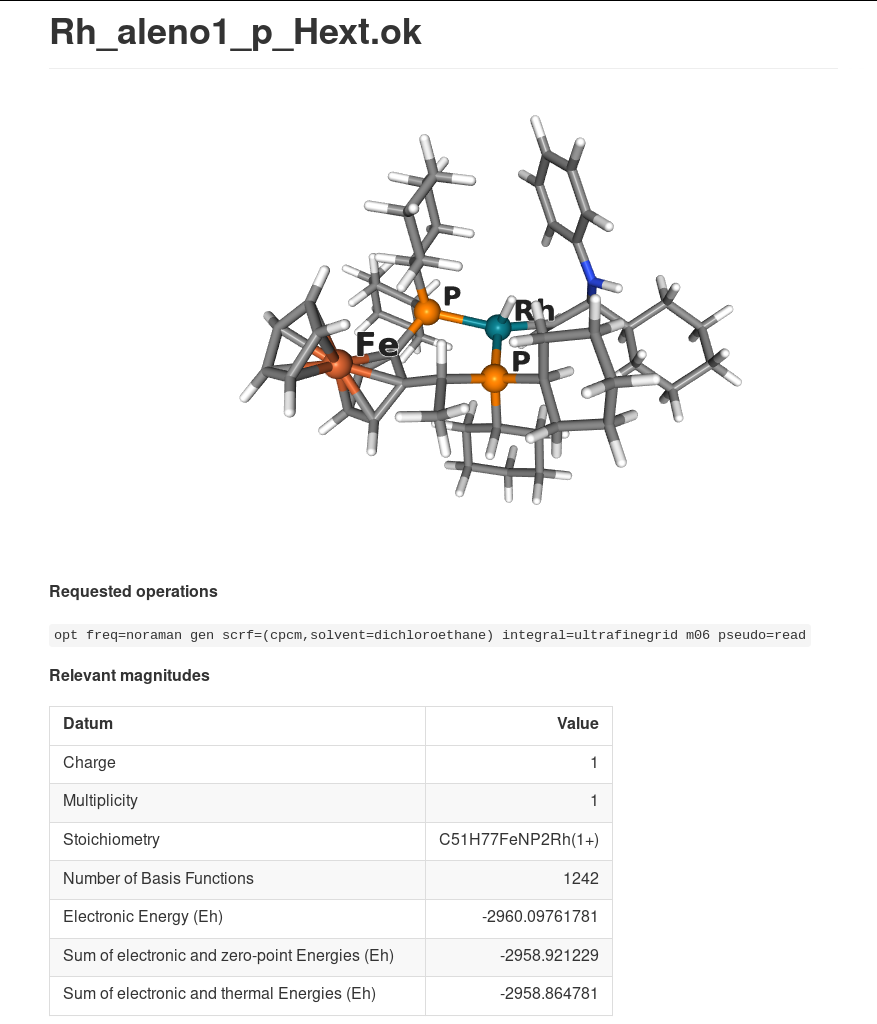
\includegraphics[width=\textwidth]{./figures/05/esigen.png}
	\cprotect\caption[ESIgen 3D report]{ESIgen can be used via a web interface and from the command line. When using the web interface (a demo is available at \href{esi.insilichem.com}{http://esi.insilichem.com}), the user only needs to upload the quantum chemistry calculation output files to the server and select the data to report. After processing the file, an interactive HTML5 preview of the 3D structure can be displayed along the requested data so the user can manually find the best orientation for a static depiction.}
	\label{fig:esigen}
\end{figure}



Both interfaces are based on the same usage principle: the user only needs to write a report template listing the requested fields as placeholders. The supplied template is then filled in with the requested data. Behind the scenes, ESIgen uses cclib\cite{cclib} to parse the computational chemistry logfiles, which means that it is compatible with wide array of suites out of the box, like Gaussian,\cite{gaussian} NWChem\cite{nwchem} or ORCA.\cite{orca} Several examples are included within the package, covering most common cases.

\subsection{Intuitive MECP calculations: EasyMECP}
% \addcontentsline{toc}{subsection}{Easy MECP calculations}

Minimum Energy Crossing Points (MECP) are defined as the consensus conformation of a molecular system that can feature low-energy minima in different spin states. A  strategy to calculate them computationally was proposed by J. N. Harvey in 1998,\cite{harvey1998} using Gaussian, GAMESS and custom Fortran routines orchestrated by shell scripts. The method and its related source code has been used widely across several research groups since then. However, setting up the MECP procedure involves recompiling the Fortran binary for each system, since it is memory allocation requires the manual specification of the number of atoms. Convergence thresholds and other hardcoded values are scattered all over the source code, which does not allow easy access to these parameters. All these technical difficulties should not concern the user.


\begin{table}[hbtp]
	\caption[EasyMECP: Technical datasheet]{EasyMECP: Technical datasheet.}
	\footnotesize
	\newcolumntype{R}{>{\hsize=.25\hsize\raggedleft\arraybackslash}X}%
	\newcolumntype{L}{>{\hsize=.75\hsize\raggedright\arraybackslash}X}%
	\newcommand{\tableheading}[1]{\multicolumn{2}{c}{\textsc{#1}}}
	\begin{tabularx}{\textwidth}{RL}
		\toprule
		%row no:1
		\tableheading{EasyMECP}\\
		\toprule
		%row no:2
		\textit{Description} & Simplified MECP calculations with Gaussian \\
		\midrule
		%row no:3
		\textit{Requirements} & Python, gfortran, Gaussian \\
		\midrule
		%row no:4
		\textit{License} & LGPL \\
		\midrule
		%row no:5
		\textit{Download} & \href{https://github.com/jaimergp/easymecp}{github.com/jaimergp/easymecp} \\
		\midrule
		%row no:6
		\textit{Documentation} & \href{https://github.com/jaimergp/easymecp}{github.com/jaimergp/easymecp} \\
		\midrule
		%row no:7
		\textit{Citation} & (In preparation) \\
		\bottomrule

	\end{tabularx}
\end{table}

Developed during the collaboration with Dr. Funes and Prof. Dr. Maseras, EasyMECP is a self-contained Python script without added dependencies that takes care of all these steps automatically. The user only needs to provide a slightly modified Gaussian input file that specifies both spin states. Under the hood, EasyMECP still uses the original Fortran code, so convergence of results is guaranteed by design. Unit-tests are provided to support this claim. Additional conveniences have been implemented such as the generation of the optimization trajectory or the automated calculation of the often-needed thermochemistry of the converged MECP structure.

\section{Conclusions $\&$  Further work}
% \addcontentsline{toc}{section}{Conclusions $\&$  Further work}
The UNIX philosophy essentially restates that subdividing a problem in smaller chunks helps in solving that problem. Simple units responsible of single tasks are easier to understand and compose together into something bigger. This approach helped devise Tangram as a cohesive suite instead of a convoluted collection of dissimilar tools. By integrating tightly with the UCSF Chimera interactive canvas, all of them can work collaboratively.

However, UCSF Chimera starts to show its age and, while PyChimera allows to use it together with more modern tools, it is only a patch and cannot be considered a definite solution. A simpler integration in the vivid Python ecosystem would be desirable. This is being solved in the new, promising version of UCSF Chimera, UCSF ChimeraX,\cite{chimerax} which provides an online repository of one-click installable extensions called the \textit{Toolshed}. ChimeraX is built on top of the same C++/Python premise, but uses the new Python 3 instead of Python 2 (which will stop receiving updates in 2020) and a different GUI library, Qt, which is easier to work with and its results are better-looking. ChimeraX is still very young and its feature set cannot be compared to the classic Chimera, but in the future this will be no longer the case. When that time comes, it will be possible to convert Tangram over to the new ChimeraX. Thanks to its modular design, the small pieces of this big puzzle could be migrated one by one, little by little, as soon as ChimeraX offers the needed features.

Developing new software is easier than changing how people work daily, though. Scientific community has proved to be very conservative about how they work, which is very paradoxical taking into account that science is all about progress. Some would argue that it is about progress, but in small steps. All the work involved in providing command-line utilities that work smarter and faster can be useless if nobody is going to use them.

For that reason, some of the tools presented in this chapter do not try to change things too much, too fast. For example, several alternative, easier-to-use MECP implementations can be found online,\cite{mecpro,mecpy,sobmecp} but people still use Harvey's. EasyMECP is only a wrapper around the time-tested Harvey's original code. It does not try to change how it works; it just changes how you use it.

Another example can be found in the Supporting Information (SI) documents. In the future, SI will consist of digital repositories that are constantly updated and discussed, as some services like Zenodo\cite{zenodo} or Figshare\cite{figshare} already provide. However, this complementary data is still being submitted as PDF documents, which are good for paper printing but not so much for data sharing. ESIgen does allow to generate PDF files from your data, but only after recommending the usage of data formats easier to share and reproduce. That will not prevent people from doing \textit{what they have always done}, but sometime in the future, slowly but surely, we might get there.
